%%%%%%%%%%%%  Generated using docx2latex.com  %%%%%%%%%%%%%%

%%%%%%%%%%%%  v2.0.0-beta  %%%%%%%%%%%%%%

\documentclass[12pt]{article}
\usepackage{amsmath}
\usepackage{latexsym}
\usepackage{amsfonts}
\usepackage[normalem]{ulem}
\usepackage{soul}
\usepackage{array}
\usepackage{amssymb}
\usepackage{extarrows}
\usepackage{graphicx}
\usepackage[backend=biber,
style=numeric,
sorting=none,
isbn=false,
doi=false,
url=false,
]{biblatex}\addbibresource{bibliography.bib}

\usepackage{subfig}
\usepackage{wrapfig}
\usepackage{wasysym}
\usepackage{enumitem}
\usepackage{adjustbox}
\usepackage{ragged2e}
\usepackage[svgnames,table]{xcolor}
\usepackage{tikz}
\usepackage{longtable}
\usepackage{changepage}
\usepackage{setspace}
\usepackage{hhline}
\usepackage{multicol}
\usepackage{tabto}
\usepackage{float}
\usepackage{multirow}
\usepackage{makecell}
\usepackage{fancyhdr}
\usepackage[toc,page]{appendix}
\usepackage[hidelinks]{hyperref}
\usetikzlibrary{shapes.symbols,shapes.geometric,shadows,arrows.meta}
\tikzset{>={Latex[width=1.5mm,length=2mm]}}
\usepackage{flowchart}\usepackage[paperheight=11.69in,paperwidth=8.27in,left=1.0in,right=1.0in,top=1.0in,bottom=1.0in,headheight=1in]{geometry}
\usepackage[utf8]{inputenc}
\usepackage[T1]{fontenc}
\TabPositions{0.5in,1.0in,1.5in,2.0in,2.5in,3.0in,3.5in,4.0in,4.5in,5.0in,5.5in,6.0in,}

\urlstyle{same}

\renewcommand{\_}{\kern-1.5pt\textunderscore\kern-1.5pt}

 %%%%%%%%%%%%  Set Depths for Sections  %%%%%%%%%%%%%%

% 1) Section
% 1.1) SubSection
% 1.1.1) SubSubSection
% 1.1.1.1) Paragraph
% 1.1.1.1.1) Subparagraph


\setcounter{tocdepth}{5}
\setcounter{secnumdepth}{5}


 %%%%%%%%%%%%  Set Depths for Nested Lists created by \begin{enumerate}  %%%%%%%%%%%%%%


\setlistdepth{9}
\renewlist{enumerate}{enumerate}{9}
		\setlist[enumerate,1]{label=\arabic*)}
		\setlist[enumerate,2]{label=\alph*)}
		\setlist[enumerate,3]{label=(\roman*)}
		\setlist[enumerate,4]{label=(\arabic*)}
		\setlist[enumerate,5]{label=(\Alph*)}
		\setlist[enumerate,6]{label=(\Roman*)}
		\setlist[enumerate,7]{label=\arabic*}
		\setlist[enumerate,8]{label=\alph*}
		\setlist[enumerate,9]{label=\roman*}

\renewlist{itemize}{itemize}{9}
		\setlist[itemize]{label=$\cdot$}
		\setlist[itemize,1]{label=\textbullet}
		\setlist[itemize,2]{label=$\circ$}
		\setlist[itemize,3]{label=$\ast$}
		\setlist[itemize,4]{label=$\dagger$}
		\setlist[itemize,5]{label=$\triangleright$}
		\setlist[itemize,6]{label=$\bigstar$}
		\setlist[itemize,7]{label=$\blacklozenge$}
		\setlist[itemize,8]{label=$\prime$}

\setlength{\topsep}{0pt}\setlength{\parindent}{0pt}

 %%%%%%%%%%%%  This sets linespacing (verticle gap between Lines) Default=1 %%%%%%%%%%%%%%


\renewcommand{\arraystretch}{1.3}


%%%%%%%%%%%%%%%%%%%% Document code starts here %%%%%%%%%%%%%%%%%%%%



\begin{document}
\begin{Center}
{\fontsize{18pt}{21.6pt}\selectfont \textbf{Short documentation on Real analysis}\par}
\end{Center}\par


\vspace{\baselineskip}

\vspace{\baselineskip}

\vspace{\baselineskip}
\begin{FlushLeft}
{\fontsize{18pt}{21.6pt}\selectfont \textbf{Question }\par}
\end{FlushLeft}\par

\begin{FlushLeft}
{\fontsize{14pt}{16.8pt}\selectfont \textbf{How to create real number from scratch?}\par}
\end{FlushLeft}\par


\vspace{\baselineskip}
\begin{FlushLeft}
{\fontsize{18pt}{21.6pt}\selectfont \textbf{What is an ordered field ?}\par}
\end{FlushLeft}\par

\begin{FlushLeft}
{\fontsize{14pt}{16.8pt}\selectfont In order to describe ordered filed first we understand what is field and what is ordered relation\par}
\end{FlushLeft}\par


\vspace{\baselineskip}
\begin{FlushLeft}
What is a field?
\end{FlushLeft}\par


\vspace{\baselineskip}
\begin{FlushLeft}
It is set f with two binary operations -> Addition , Multiplication 
\end{FlushLeft}\par


\vspace{\baselineskip}
\begin{FlushLeft}
Any set which satisfy asscotivity, {\fontsize{10pt}{12.0pt}\selectfont commutativity, distributy,commutativity, inverse then such called call set of field OR we can say these are the property of field set\par}
\end{FlushLeft}\par


\vspace{\baselineskip}
\begin{FlushLeft}
{\fontsize{10pt}{12.0pt}\selectfont Example: Set of rational number, Set of Real numbers\par}
\end{FlushLeft}\par


\vspace{\baselineskip}
\begin{FlushLeft}
{\fontsize{10pt}{12.0pt}\selectfont  \par}
\end{FlushLeft}\par


\vspace{\baselineskip}

\vspace{\baselineskip}
\begin{FlushLeft}
\textbf{Answer:}
\end{FlushLeft}\par

\begin{FlushLeft}
\textbf{A field(f + .) is an ordered field if the following properties are satisfied}
\end{FlushLeft}\par


\vspace{\baselineskip}
\begin{enumerate}
	\item \textbf{Trichotomy property}\par

	\item \textbf{Transitive property}\par

	\item \textbf{Addition composition}\par

	\item \textbf{Multiplication composition}
\end{enumerate}\par


\vspace{\baselineskip}
\begin{FlushLeft}
Some other points:
\end{FlushLeft}\par


\vspace{\baselineskip}
\begin{FlushLeft}
Supremum: In simple words least upper bound is called supremum
\end{FlushLeft}\par

\begin{FlushLeft}
Infimum:\ \ Greatest lower  bound 
\end{FlushLeft}\par


\vspace{\baselineskip}

\vspace{\baselineskip}
\textbf{complete} \textbf{ordered field:}\par


\vspace{\baselineskip}
\textbf{When an ordered field is bounded above and bounded below. In other words}\par

\textbf{When\ supremum and infimum  values are coming in ordered field then we will say that field is complete ordered field}\par


\vspace{\baselineskip}

\vspace{\baselineskip}
\begin{FlushLeft}
Construction of real number
\end{FlushLeft}\par


\vspace{\baselineskip}
\begin{enumerate}
	\item Synthetic approach (Reference from wikipedia)\par


\vspace{\baselineskip}
\begin{FlushLeft}
Synthetic approach defined real number system as a \textbf{complete} \textbf{ordered field} 
\end{FlushLeft}\par


\vspace{\baselineskip}
\begin{FlushLeft}
Such that real number system consist of set R {\fontsize{10pt}{12.0pt}\selectfont \textcolor[HTML]{222222}{two distinct elements 0 and 1 of \textbf{R}, two \href{https://en.wikipedia.org/wiki/Binary_operation}{binary operations} + and $ \times $  on \textbf{R.}}\par}
\end{FlushLeft}\par


\vspace{\baselineskip}

\vspace{\baselineskip}

\vspace{\baselineskip}

\vspace{\baselineskip}

\vspace{\baselineskip}
	\item Cauchy Sequence 
\end{enumerate}\par

\begin{FlushLeft}
Whats is cauchy sequence ?
\end{FlushLeft}\par


\vspace{\baselineskip}
\begin{FlushLeft}
A\ sequence is said to be a cauchy sequence  for every epsilon greater than zero
\end{FlushLeft}\par

\begin{FlushLeft}
There\ is\ a\ positive\ integer\ m\ \ \ \       \textit{m}, \textit{n} > \textit{N} then $ \vert $ \textit{a\textsubscript{m}}- \textit{a\textsubscript{n}}$ \vert $  < \textit{$ \varepsilon $ }. For all m>n
\end{FlushLeft}\par


\vspace{\baselineskip}

\vspace{\baselineskip}

\vspace{\baselineskip}

\vspace{\baselineskip}

\vspace{\baselineskip}
\begin{FlushLeft}
-------------------------------------------------------------------------
\end{FlushLeft}\par


\vspace{\baselineskip}

\vspace{\baselineskip}

\vspace{\baselineskip}
\begin{FlushLeft}
First we will construct Natural Numbers:
\end{FlushLeft}\par


\vspace{\baselineskip}
\begin{FlushLeft}
Constructing Real numbers with Peano’s Axiom
\end{FlushLeft}\par

\begin{FlushLeft}
\uline{Axioms:}
\end{FlushLeft}\par

\begin{enumerate}
	\item There exist a natural number 1\par

	\item If\ a is a natural number, then its successor  s(a) = a+1 is also a natural number.\par

	\item 1 is not the successor is any natural number\par

	\item If two numbers have the same successor then they must be the same number\par

	\item Given a set S, if 1 belongs to S and contains the successor of any number in S then S must contain all of the natural numbers.
\end{enumerate}\par


\vspace{\baselineskip}

\vspace{\baselineskip}

\vspace{\baselineskip}

\vspace{\baselineskip}
\begin{FlushLeft}
----------------------------------
\end{FlushLeft}\par


\vspace{\baselineskip}
\begin{FlushLeft}
{\fontsize{14pt}{16.8pt}\selectfont \textbf{Hol Light}\par}
\end{FlushLeft}\par


\vspace{\baselineskip}
\begin{FlushLeft}
{\fontsize{14pt}{16.8pt}\selectfont \tab  \tab  \tab  \tab  \tab \par}
\end{FlushLeft}\par

1.Referencing link for HOL LIGHT ->\href{https://github.com/jrh13/hol-light/}{ }\href{https://github.com/jrh13/hol-light/}{\textcolor[HTML]{0000E9}{\ul{https://github.com/jrh13/hol-light/}}}\par

2. Getting errors -> Cannot find file camlp5o.cma and Cannot find file /Users/craftandcode/pa\_j.cmo.\par

3.Resolved above by using\par

$\#$ require $``$camlp5$"$  in utop\par

And running utop from cloned hol-light folder\par


\vspace{\baselineskip}
\textcolor[HTML]{1B1F22}{4. HOL Basics}\par


\vspace{\baselineskip}
\textcolor[HTML]{1B1F22}{a.Terms are enclosed in back quotes $``$`$"$  ex. `x+1`}\par

\textcolor[HTML]{1B1F22}{b.subst will be used to replace a term by another}\par

\textcolor[HTML]{1B1F22}{ex. subst [`y + 2`,`x:num`] `x + 5 $\ast$  x`;;}\par


\vspace{\baselineskip}
\textcolor[HTML]{1B1F22}{c.Theorem has type $``$thm$"$ }\par

\textcolor[HTML]{1B1F22}{eg1. Checking the reflexivity of equality operator}\par

\textcolor[HTML]{1B1F22}{$\#$  REFL `x:real`;;}\par

\textcolor[HTML]{1B1F22}{returns -> }val it : thm = $ \vert $ - x = x\par


\vspace{\baselineskip}
eg2. Assume is used to assume a statement\par

$\#$  ASSUME ` x = 2`;;\par

returns -> val th2 : thm = x = 2 $ \vert $ - x = 2\par


\vspace{\baselineskip}
eg3. INST is used to instantiate a variable in a theorem to some value\par

let th3 = INST [`0`,`x:num`] th1;;\par

returns -> val th3 : thm = $ \vert $ - 0 + y = 0 <=> 0 + y = 0\par


\vspace{\baselineskip}
\textcolor[HTML]{1B1F22}{eg4. concl is used to conclude a theorem}\par

concl th1;;\par

returns -> val it : term = `x + y = 0 <=> x + y = 0`\par


\vspace{\baselineskip}

\vspace{\baselineskip}

\vspace{\baselineskip}
\begin{FlushLeft}
{\fontsize{14pt}{16.8pt}\selectfont Some Issues faced:\par}
\end{FlushLeft}\par


\vspace{\baselineskip}


%%%%%%%%%%%%%%%%%%%% Figure/Image No: 1 starts here %%%%%%%%%%%%%%%%%%%%

\begin{figure}[H]
	\begin{FlushLeft}		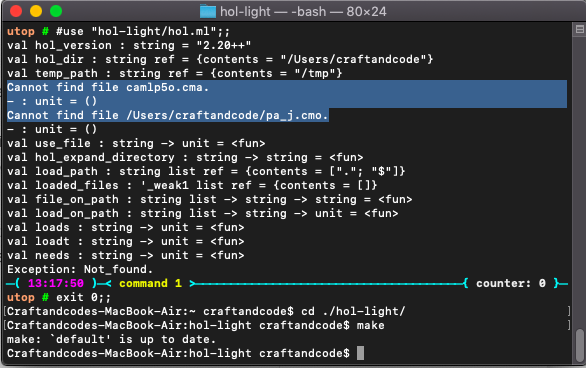
\includegraphics[width=6.1in,height=3.83in]{./media/image19.png}
	\end{FlushLeft}\end{figure}


%%%%%%%%%%%%%%%%%%%% Figure/Image No: 1 Ends here %%%%%%%%%%%%%%%%%%%%

\par



%%%%%%%%%%%%%%%%%%%% Figure/Image No: 2 starts here %%%%%%%%%%%%%%%%%%%%

\begin{figure}[H]
	\begin{FlushLeft}		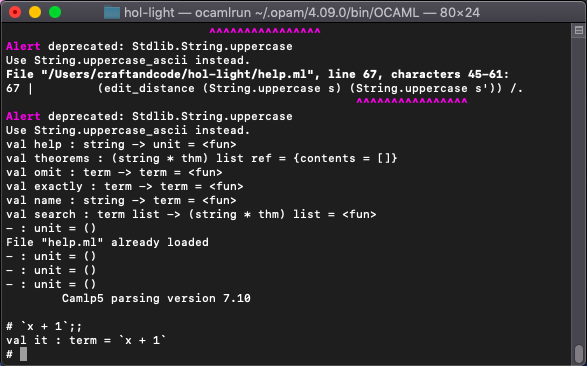
\includegraphics[width=6.11in,height=3.81in]{./media/image17.png}
	\end{FlushLeft}\end{figure}


%%%%%%%%%%%%%%%%%%%% Figure/Image No: 2 Ends here %%%%%%%%%%%%%%%%%%%%

\par



%%%%%%%%%%%%%%%%%%%% Figure/Image No: 3 starts here %%%%%%%%%%%%%%%%%%%%

\begin{figure}[H]
	\begin{Center}
		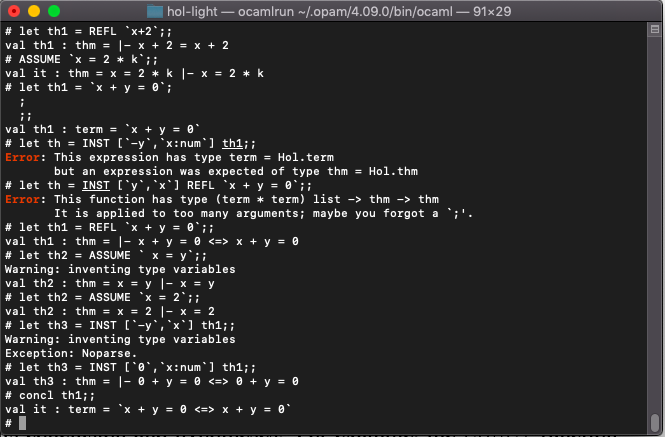
\includegraphics[width=6.27in,height=4.12in]{./media/image24.png}
	\end{Center}
\end{figure}


%%%%%%%%%%%%%%%%%%%% Figure/Image No: 3 Ends here %%%%%%%%%%%%%%%%%%%%

\par


\vspace{\baselineskip}


%%%%%%%%%%%%%%%%%%%% Figure/Image No: 4 starts here %%%%%%%%%%%%%%%%%%%%

\begin{figure}[H]
	\begin{Center}
		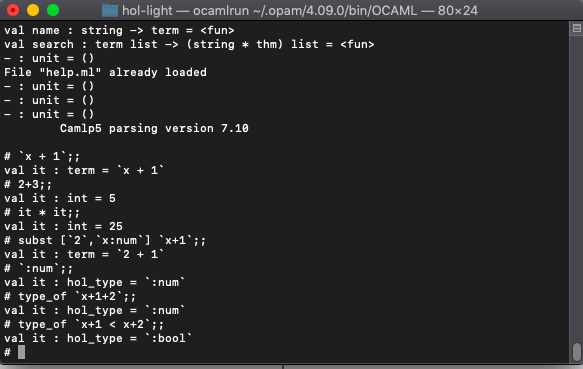
\includegraphics[width=6.07in,height=3.84in]{./media/image13.png}
	\end{Center}
\end{figure}


%%%%%%%%%%%%%%%%%%%% Figure/Image No: 4 Ends here %%%%%%%%%%%%%%%%%%%%

\par


\vspace{\baselineskip}

\vspace{\baselineskip}

\vspace{\baselineskip}

\vspace{\baselineskip}

\vspace{\baselineskip}

\vspace{\baselineskip}

\vspace{\baselineskip}

\vspace{\baselineskip}

\vspace{\baselineskip}

\vspace{\baselineskip}

\vspace{\baselineskip}

\vspace{\baselineskip}

\vspace{\baselineskip}

\vspace{\baselineskip}

\vspace{\baselineskip}

\vspace{\baselineskip}

\vspace{\baselineskip}

\vspace{\baselineskip}

\vspace{\baselineskip}

\vspace{\baselineskip}

\vspace{\baselineskip}
\begin{FlushLeft}
{\fontsize{14pt}{16.8pt}\selectfont \textbf{6/01/2020}\par}
\end{FlushLeft}\par


\vspace{\baselineskip}
{\fontsize{14pt}{16.8pt}\selectfont Some basic definition:\par}\par


\vspace{\baselineskip}

\vspace{\baselineskip}
{\fontsize{14pt}{16.8pt}\selectfont Least\ element:  Let A is subset of Q where Q is a set of all Rational number, r belongs to Q then r is said to be least element of A only if\par}\par

\begin{enumerate}
	\item {\fontsize{14pt}{16.8pt}\selectfont r belongs to A\par}\par

	\item {\fontsize{14pt}{16.8pt}\selectfont r<= x , for all x belongs to A\par}
\end{enumerate}\par


\vspace{\baselineskip}
{\fontsize{14pt}{16.8pt}\selectfont Largest\ element:  Let A is subset of Q where Q is a set of all Rational number, u belongs to Q then u is said to be Largest element of A only if\par}\par

\begin{enumerate}
	\item {\fontsize{14pt}{16.8pt}\selectfont u belongs to A\par}\par

	\item {\fontsize{14pt}{16.8pt}\selectfont u>= x, for all x belongs A\par}
\end{enumerate}\par


\vspace{\baselineskip}

\vspace{\baselineskip}
\begin{FlushLeft}
{\fontsize{14pt}{16.8pt}\selectfont (This definition is in my own words may be not like standard definition)\par}
\end{FlushLeft}\par


\vspace{\baselineskip}
\begin{FlushLeft}
{\fontsize{14pt}{16.8pt}\selectfont \textbf{Dedekind Cuts}:\ \ Since the set of rational is an ordered field so  we can arrange this set of rational number Q on number line. Suppose we mark a cut P on that number line such that it divides number line in two parts or in two sub set of Q.\par}
\end{FlushLeft}\par


\vspace{\baselineskip}

\vspace{\baselineskip}


%%%%%%%%%%%%%%%%%%%% Figure/Image No: 5 starts here %%%%%%%%%%%%%%%%%%%%

\begin{figure}[H]
	\begin{FlushLeft}		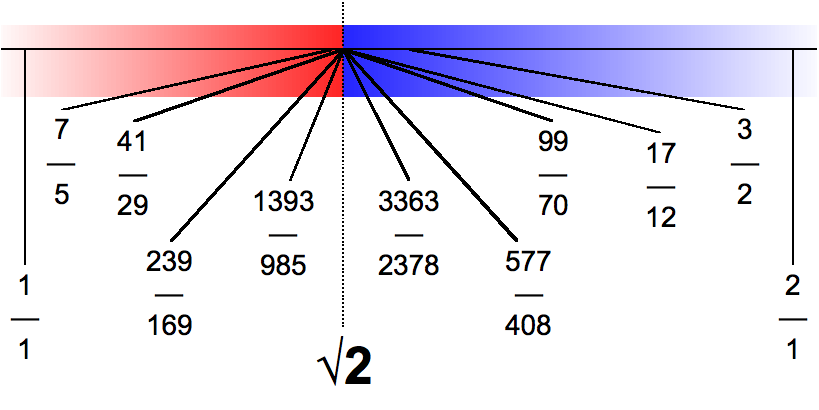
\includegraphics[width=6.3in,height=1.65in]{./media/image1.png}
	\end{FlushLeft}\end{figure}


%%%%%%%%%%%%%%%%%%%% Figure/Image No: 5 Ends here %%%%%%%%%%%%%%%%%%%%

\par


\vspace{\baselineskip}
\begin{FlushLeft}
{\fontsize{14pt}{16.8pt}\selectfont What we will have after dividing the number line:\par}
\end{FlushLeft}\par

\begin{enumerate}
	\item {\fontsize{14pt}{16.8pt}\selectfont There will be two part one on left hand $``$L$"$  called lower class element and other on Right hand side $``$U$"$  called Upper class elements.\par}\par

	\item {\fontsize{14pt}{16.8pt}\selectfont Lower class $``$L$"$  elements are smaller that Upper class elements $``$U$"$ .\par}\par

	\item {\fontsize{14pt}{16.8pt}\selectfont There are two possibilities for cut $``$P$"$ . It could be Rational number or irrational number.\par}\par

	\item {\fontsize{14pt}{16.8pt}\selectfont If P is irrational number then all rational either belongs to $``$L$"$  or belongs $``$U$"$  and P itself become the largest element of U\par}\par

	\item {\fontsize{14pt}{16.8pt}\selectfont If cut P is a rational number then means P is in the form of p/q\par}
\end{enumerate}\par

\begin{adjustwidth}{0.5in}{0.0in}
\begin{FlushLeft}
{\fontsize{14pt}{16.8pt}\selectfont Then P belongs to $``$U$"$ . Means P will be element of Right hand set\par}
\end{FlushLeft}\par

\end{adjustwidth}


\vspace{\baselineskip}

\vspace{\baselineskip}

\vspace{\baselineskip}

\vspace{\baselineskip}

\vspace{\baselineskip}

\vspace{\baselineskip}

\vspace{\baselineskip}
\begin{FlushLeft}
{\fontsize{14pt}{16.8pt}\selectfont \textbf{Standard Definition from above explanation}\par}
\end{FlushLeft}\par


\vspace{\baselineskip}
{\fontsize{11pt}{13.2pt}\selectfont \textcolor[HTML]{161616}{A Dedekind }{\fontsize{14pt}{16.8pt}\selectfont \textcolor[HTML]{161616}{cut }{\fontsize{13pt}{15.6pt}\selectfont \textcolor[HTML]{161616}{x = (L, U)\textit{ }in Q is a pair of subset L,U of Q satisfying the following condition}\par}\par}\par}\par


\vspace{\baselineskip}
\begin{enumerate}
	\item {\fontsize{13pt}{15.6pt}\selectfont \textcolor[HTML]{161616}{L\ union U = Q ,  L intersection U = $ \{ $ $ \} $ , L and U are non empty sets}\par}\par

	\item {\fontsize{13pt}{15.6pt}\selectfont \textcolor[HTML]{161616}{If l belongs L and u belongs U then l<u}\par}\par

	\item {\fontsize{13pt}{15.6pt}\selectfont \textcolor[HTML]{161616}{L\ will not have the largest element  }\par}
\end{enumerate}\par


\vspace{\baselineskip}

\vspace{\baselineskip}

\vspace{\baselineskip}

\vspace{\baselineskip}
\begin{FlushLeft}
{\fontsize{14pt}{16.8pt}\selectfont Hol Light Study:\par}
\end{FlushLeft}\par


\vspace{\baselineskip}

\vspace{\baselineskip}
\textbf{\uline{Ref. Book }-> Hol Light (John Horrison)}\par

\textbf{\uline{ }}\par

\textbf{\uline{Derived rules}}\par

Summary -> Theorem that needs to be proved only by rearrangement/simplification of terms can be proved by ARITH\_RULE\par

Eg. {\fontsize{14pt}{16.8pt}\selectfont $\#$  ARITH\_RULE `(a$\ast$ x+b$\ast$ x) = x$\ast$ (a+b)`;;\par}\par

{\fontsize{14pt}{16.8pt}\selectfont Returns -> val it : thm = $ \vert $ - a $\ast$  x + b $\ast$  x = x $\ast$  (a + b)\par}\par

{\fontsize{14pt}{16.8pt}\selectfont  \par}\par

{\fontsize{14pt}{16.8pt}\selectfont \textbf{\uline{Propositional Logic}}\par}\par

{\fontsize{14pt}{16.8pt}\selectfont Notations used\par}\par



%%%%%%%%%%%%%%%%%%%% Table No: 1 starts here %%%%%%%%%%%%%%%%%%%%


\begin{table}[H]
 			\centering
\begin{tabular}{p{0.25in}p{0.37in}p{1.71in}}
%row no:1
\multicolumn{1}{p{0.25in}}{{\fontsize{13pt}{15.6pt}\selectfont $\bot$ }} & 
\multicolumn{1}{p{0.37in}}{{\fontsize{13pt}{15.6pt}\selectfont F}} & 
\multicolumn{1}{p{1.71in}}{{\fontsize{13pt}{15.6pt}\selectfont Falsity}} \\
\hhline{~~~}
%row no:2
\multicolumn{1}{p{0.25in}}{{\fontsize{13pt}{15.6pt}\selectfont ⊤}} & 
\multicolumn{1}{p{0.37in}}{{\fontsize{13pt}{15.6pt}\selectfont T}} & 
\multicolumn{1}{p{1.71in}}{{\fontsize{13pt}{15.6pt}\selectfont Truth}} \\
\hhline{~~~}
%row no:3
\multicolumn{1}{p{0.25in}}{{\fontsize{13pt}{15.6pt}\selectfont ¬}} & 
\multicolumn{1}{p{0.37in}}{{\fontsize{13pt}{15.6pt}\selectfont ̃}} & 
\multicolumn{1}{p{1.71in}}{{\fontsize{13pt}{15.6pt}\selectfont Not}} \\
\hhline{~~~}
%row no:4
\multicolumn{1}{p{0.25in}}{{\fontsize{13pt}{15.6pt}\selectfont $\wedge$ }} & 
\multicolumn{1}{p{0.37in}}{{\fontsize{13pt}{15.6pt}\selectfont /$\textbackslash$ }} & 
\multicolumn{1}{p{1.71in}}{{\fontsize{13pt}{15.6pt}\selectfont And}} \\
\hhline{~~~}
%row no:5
\multicolumn{1}{p{0.25in}}{{\fontsize{13pt}{15.6pt}\selectfont $ \vee $ }} & 
\multicolumn{1}{p{0.37in}}{{\fontsize{13pt}{15.6pt}\selectfont $\textbackslash$ /}} & 
\multicolumn{1}{p{1.71in}}{{\fontsize{13pt}{15.6pt}\selectfont Or}} \\
\hhline{~~~}
%row no:6
\multicolumn{1}{p{0.25in}}{{\fontsize{13pt}{15.6pt}\selectfont $ \Rightarrow $ }} & 
\multicolumn{1}{p{0.37in}}{{\fontsize{13pt}{15.6pt}\selectfont ==>}} & 
\multicolumn{1}{p{1.71in}}{{\fontsize{13pt}{15.6pt}\selectfont Implies (‘if ...then ...’)}} \\
\hhline{~~~}
%row no:7
\multicolumn{1}{p{0.25in}}{{\fontsize{13pt}{15.6pt}\selectfont $ \Leftrightarrow $ }} & 
\multicolumn{1}{p{0.37in}}{{\fontsize{13pt}{15.6pt}\selectfont <=>}} & 
\multicolumn{1}{p{1.71in}}{{\fontsize{13pt}{15.6pt}\selectfont Iff (‘...if and only if ...’)}} \\
\hhline{~~~}

\end{tabular}
 \end{table}


%%%%%%%%%%%%%%%%%%%% Table No: 1 ends here %%%%%%%%%%%%%%%%%%%%

{\fontsize{14pt}{16.8pt}\selectfont A => B is {\fontsize{13pt}{15.6pt}\selectfont ¬A $ \vee $  B\par}\par}\par

{\fontsize{13pt}{15.6pt}\selectfont A $ \Leftrightarrow $  B is (A => B) $\wedge$  (B => A)\par}\par

{\fontsize{13pt}{15.6pt}\selectfont  \par}\par

{\fontsize{13pt}{15.6pt}\selectfont To get the precedence and associativity of an infix operators .\par}\par

{\fontsize{14pt}{16.8pt}\selectfont 1.infixes();;\par}\par

{\fontsize{13pt}{15.6pt}\selectfont It will give all the infix operators along with precedence and associativity\par}\par

 \par

2.get\_infix\_status "op$"$ ;;\par

It will give the precedence and associativity of operator $``$op$"$ \par

Eg . get\_infix\_status $``$==>$"$ ;;\par

Returns -> {\fontsize{14pt}{16.8pt}\selectfont val it : int $\ast$  string = (4, "right")\par}\par

 \par

We can make any other symbol as infix or can change precedence existing infixes using\par

{\fontsize{13pt}{15.6pt}\selectfont parse\_as\_infix($``$op$"$ ,(precedence,$"$ Associativity$"$ ))\par}\par

{\fontsize{13pt}{15.6pt}\selectfont Eg. parse\_as\_infix($``$<>$"$ ,(12,$"$ right$"$ ));\par}\par

{\fontsize{9pt}{10.8pt}\selectfont  \par}\par

{\fontsize{13pt}{15.6pt}\selectfont \textbf{\uline{Tautology}} :- A tautology is a formula or assertion that is true in every case.\par}\par

{\fontsize{13pt}{15.6pt}\selectfont Eg. x = y or x<> y\par}\par

{\fontsize{13pt}{15.6pt}\selectfont Eg.\textcolor[HTML]{1A1A1A}{"The ball is all green, or the ball is not all green"}\par}\par

{\fontsize{13pt}{15.6pt}\selectfont Ref->\href{https://en.wikipedia.org/wiki/Tautology_(logic)}{ }\href{https://en.wikipedia.org/wiki/Tautology_(logic)}{\textcolor[HTML]{0000E9}{\ul{https://en.wikipedia.org/wiki/Tautology\_(logic)}}}\par}\par

\textcolor[HTML]{0000E9}{\uline{ }}\par

{\fontsize{13pt}{15.6pt}\selectfont TAUT will prove the tautologies directly\par}\par

{\fontsize{13pt}{15.6pt}\selectfont Eg.\ TAUT  `p $\textbackslash$ / $ \sim $ p `;;\par}\par

{\fontsize{13pt}{15.6pt}\selectfont Returns-> {\fontsize{14pt}{16.8pt}\selectfont val it : term = `p $\textbackslash$ / $ \sim $ p`\par}\par}\par

{\fontsize{14pt}{16.8pt}\selectfont Eg. TAUT {\fontsize{13pt}{15.6pt}\selectfont  `p $\textbackslash$ / p `;;\par}\par}\par

{\fontsize{13pt}{15.6pt}\selectfont Returns -> {\fontsize{14pt}{16.8pt}\selectfont Exception: Failure "TAC\_PROOF: Unsolved goals".\par}\par}\par

 \par

{\fontsize{13pt}{15.6pt}\selectfont Some other examples\par}\par

{\fontsize{13pt}{15.6pt}\selectfont 1.De Morgan’s law\par}\par

{\fontsize{13pt}{15.6pt}\selectfont a.\  TAUT `$ \sim $ (p /$\textbackslash$  q) <=> $ \sim $ p $\textbackslash$ / $ \sim $ q`;;\par}\par

{\fontsize{13pt}{15.6pt}\selectfont val\ it\ : thm = $ \vert $ - $ \sim $ (p /$\textbackslash$  q) <=>  $ \sim $ p $\textbackslash$ /  $ \sim $ q\par}\par

{\fontsize{13pt}{15.6pt}\selectfont b. TAUT `$ \sim $ (p $\textbackslash$ / q) <=> $ \sim $ p /$\textbackslash$  $ \sim $ q`;;\par}\par

{\fontsize{13pt}{15.6pt}\selectfont val it : thm = $ \vert $ - $ \sim $ (p $\textbackslash$ / q) <=> $ \sim $ p /$\textbackslash$  $ \sim $ q\par}\par

{\fontsize{9pt}{10.8pt}\selectfont  \par}\par

{\fontsize{13pt}{15.6pt}\selectfont 2.Peirce’s Law\par}\par

{\fontsize{13pt}{15.6pt}\selectfont a.\  TAUT `((p ==> q) ==> p) ==> p`;;\par}\par

{\fontsize{14pt}{16.8pt}\selectfont val it : thm = $ \vert $ - ((p ==> q) ==> p) ==> p\par}\par

 \par

3. {\fontsize{13pt}{15.6pt}\selectfont \ TAUT  `x < 1 /$\textbackslash$  y > 0 ==> x < 1`;;\par}\par

{\fontsize{14pt}{16.8pt}\selectfont val it : thm = $ \vert $ - x < 1 /$\textbackslash$  y > 0 ==> x < 1\par}\par

{\fontsize{14pt}{16.8pt}\selectfont  \par}\par

{\fontsize{14pt}{16.8pt}\selectfont 4. {\fontsize{13pt}{15.6pt}\selectfont TAUT\  `0 < x /$\textbackslash$  x < 7 ==> 1 <= x /$\textbackslash$  x <= 6`;;\par}\par}\par

{\fontsize{14pt}{16.8pt}\selectfont Exception: Failure "TAC\_PROOF: Unsolved goals$"$ .\par}\par

{\fontsize{14pt}{16.8pt}\selectfont Can be resolved by using ARITH\_RULE which analyses arithmetic content\par}\par

{\fontsize{13pt}{15.6pt}\selectfont So ARITH\_RULE `0 < x /$\textbackslash$  x < 7 ==> 1 <= x /$\textbackslash$  x <= 6`;; will work here\par}\par

{\fontsize{9pt}{10.8pt}\selectfont  \par}\par


\vspace{\baselineskip}

\vspace{\baselineskip}

\vspace{\baselineskip}


%%%%%%%%%%%%%%%%%%%% Figure/Image No: 6 starts here %%%%%%%%%%%%%%%%%%%%

\begin{figure}[H]
	\begin{FlushLeft}		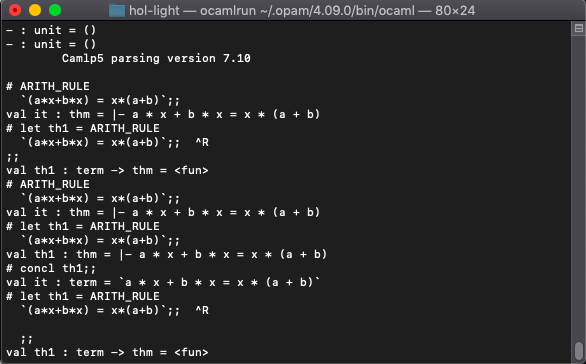
\includegraphics[width=6.1in,height=3.79in]{./media/image15.png}
	\end{FlushLeft}\end{figure}


%%%%%%%%%%%%%%%%%%%% Figure/Image No: 6 Ends here %%%%%%%%%%%%%%%%%%%%

\par


\vspace{\baselineskip}

\vspace{\baselineskip}


%%%%%%%%%%%%%%%%%%%% Figure/Image No: 7 starts here %%%%%%%%%%%%%%%%%%%%

\begin{figure}[H]
	\begin{FlushLeft}		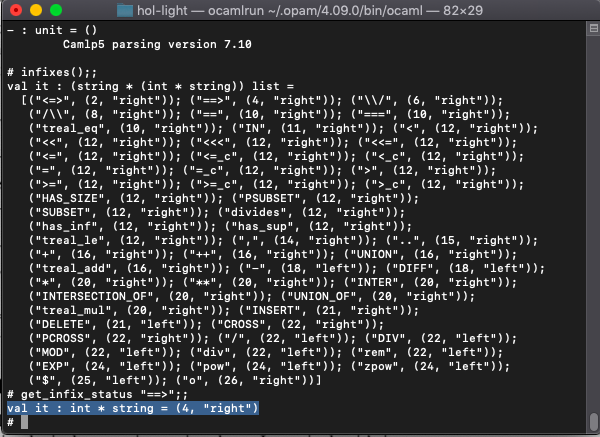
\includegraphics[width=6.25in,height=4.55in]{./media/image23.png}
	\end{FlushLeft}\end{figure}


%%%%%%%%%%%%%%%%%%%% Figure/Image No: 7 Ends here %%%%%%%%%%%%%%%%%%%%

\par


\vspace{\baselineskip}

\vspace{\baselineskip}


%%%%%%%%%%%%%%%%%%%% Figure/Image No: 8 starts here %%%%%%%%%%%%%%%%%%%%

\begin{figure}[H]
	\begin{FlushLeft}		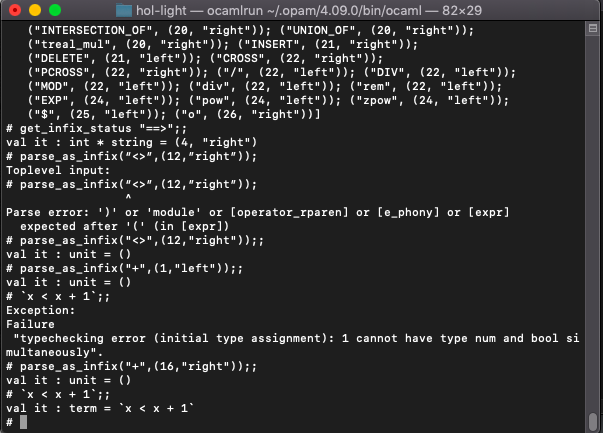
\includegraphics[width=6.27in,height=4.5in]{./media/image20.png}
	\end{FlushLeft}\end{figure}


%%%%%%%%%%%%%%%%%%%% Figure/Image No: 8 Ends here %%%%%%%%%%%%%%%%%%%%

\par


\vspace{\baselineskip}

\vspace{\baselineskip}


%%%%%%%%%%%%%%%%%%%% Figure/Image No: 9 starts here %%%%%%%%%%%%%%%%%%%%

\begin{figure}[H]
	\begin{FlushLeft}		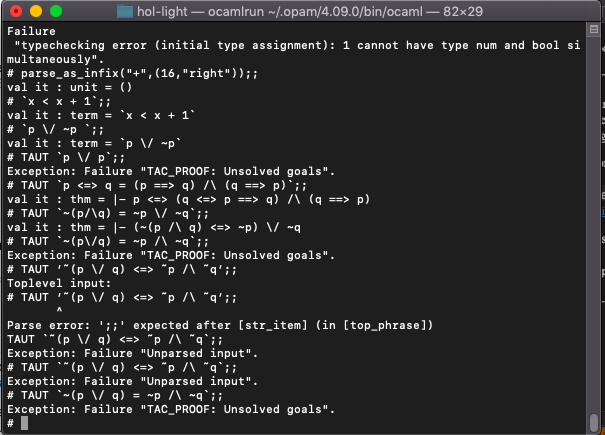
\includegraphics[width=6.27in,height=4.51in]{./media/image25.png}
	\end{FlushLeft}\end{figure}


%%%%%%%%%%%%%%%%%%%% Figure/Image No: 9 Ends here %%%%%%%%%%%%%%%%%%%%

\par


\vspace{\baselineskip}


%%%%%%%%%%%%%%%%%%%% Figure/Image No: 10 starts here %%%%%%%%%%%%%%%%%%%%

\begin{figure}[H]
	\begin{FlushLeft}		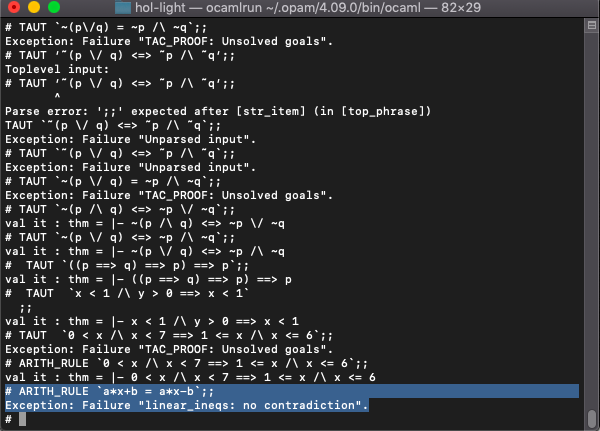
\includegraphics[width=6.25in,height=4.49in]{./media/image22.png}
	\end{FlushLeft}\end{figure}


%%%%%%%%%%%%%%%%%%%% Figure/Image No: 10 Ends here %%%%%%%%%%%%%%%%%%%%

\par


\vspace{\baselineskip}

\vspace{\baselineskip}

\vspace{\baselineskip}


%%%%%%%%%%%%%%%%%%%% Figure/Image No: 11 starts here %%%%%%%%%%%%%%%%%%%%

\begin{figure}[H]
	\begin{FlushLeft}		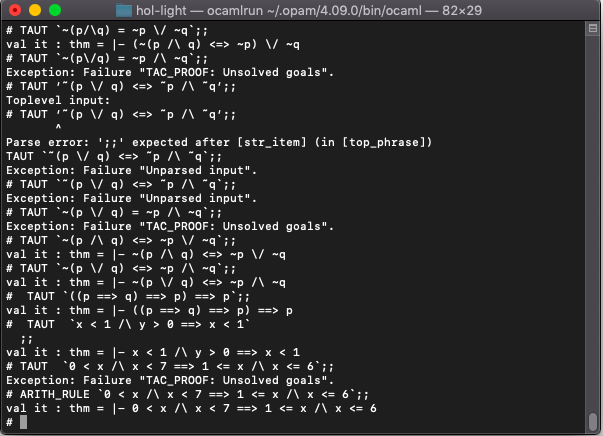
\includegraphics[width=6.27in,height=4.53in]{./media/image21.png}
	\end{FlushLeft}\end{figure}


%%%%%%%%%%%%%%%%%%%% Figure/Image No: 11 Ends here %%%%%%%%%%%%%%%%%%%%

\par


\vspace{\baselineskip}

\vspace{\baselineskip}

\vspace{\baselineskip}
\begin{FlushLeft}
{\fontsize{14pt}{16.8pt}\selectfont \textbf{07/01/2020}\par}
\end{FlushLeft}\par


\vspace{\baselineskip}
\begin{FlushLeft}
{\fontsize{14pt}{16.8pt}\selectfont \tab  \tab  \tab  \tab \par}
\end{FlushLeft}\par

{\fontsize{13pt}{15.6pt}\selectfont \textbf{\uline{Equations and Functions}}\par}\par


\vspace{\baselineskip}
{\fontsize{13pt}{15.6pt}\selectfont HOL Terms types\par}\par

{\fontsize{13pt}{15.6pt}\selectfont 1.Variable -> `x:bool` , `n:num`\par}\par

{\fontsize{13pt}{15.6pt}\selectfont 2.Constants -> `T` (True) , `F` (False)\par}\par

{\fontsize{13pt}{15.6pt}\selectfont 3.Applications\par}\par

{\fontsize{13pt}{15.6pt}\selectfont 4.Abstractions\par}\par


\vspace{\baselineskip}
{\fontsize{13pt}{15.6pt}\selectfont \textbf{\uline{Applications}} -> Application of a function to an argument , which is a composite term built from subterms for the function and argument.\par}\par

{\fontsize{13pt}{15.6pt}\selectfont Eg. `$ \sim $ p` is an application of the constant denoting the negation operator to a Boolean variable\par}\par

{\fontsize{13pt}{15.6pt}\selectfont We use customary jargon \textit{rator} (ope-gator = function ) and \textit{rand }(ope-rand = argument) for two components of an application.\par}\par

{\fontsize{13pt}{15.6pt}\selectfont eg. rator `$ \sim $ p`;;\par}\par

{\fontsize{13pt}{15.6pt}\selectfont returns -> val it : term = `($ \sim $ )`\par}\par

{\fontsize{13pt}{15.6pt}\selectfont eg. rand `$ \sim $ p`;;\par}\par

{\fontsize{13pt}{15.6pt}\selectfont returns -> val it : term = `p`\par}\par


\vspace{\baselineskip}
{\fontsize{13pt}{15.6pt}\selectfont \textbf{\uline{Curried functions}} -> Function may take one argument and yield another function and this can be exploited to get the same effect.\par}\par

{\fontsize{13pt}{15.6pt}\selectfont eg. a+b can be represented as ((+) a)(b)\par}\par

{\fontsize{13pt}{15.6pt}\selectfont eg. let successor = (+) 1;;\par}\par

{\fontsize{13pt}{15.6pt}\selectfont successor 4;;\par}\par

{\fontsize{13pt}{15.6pt}\selectfont returns -> val it : int = 5\par}\par


\vspace{\baselineskip}
{\fontsize{13pt}{15.6pt}\selectfont Function application associates to the left, so \textit{f a b} means \textit{(f a) b}\par}\par


\vspace{\baselineskip}
{\fontsize{13pt}{15.6pt}\selectfont \textbf{\uline{Pairing}} -> Complex terms can be represented as for an example\par}\par

{\fontsize{13pt}{15.6pt}\selectfont eg. `(==>) ((=) ((+) x y) z) (P z)`;;\par}\par

{\fontsize{13pt}{15.6pt}\selectfont returns -> val it : term = `x + y = z ==> P z`\par}\par


\vspace{\baselineskip}
{\fontsize{13pt}{15.6pt}\selectfont Ordered Pair can be constructed by binary infix operator $``$,$"$ \par}\par

{\fontsize{13pt}{15.6pt}\selectfont eg. `1,2`\par}\par

{\fontsize{13pt}{15.6pt}\selectfont -> val it : term = `1,2`\par}\par

{\fontsize{13pt}{15.6pt}\selectfont type\_of it;;\par}\par

{\fontsize{13pt}{15.6pt}\selectfont -> val it : hol\_type = `:num$\#$ num`\par}\par


\vspace{\baselineskip}
{\fontsize{13pt}{15.6pt}\selectfont mk\_comb -> builds an application out of function and argument, taking pair of arguments.\par}\par

{\fontsize{13pt}{15.6pt}\selectfont eg. mk\_comb(`(+) x`,`y:num`);;\par}\par

{\fontsize{14pt}{16.8pt}\selectfont —{\fontsize{13pt}{15.6pt}\selectfont > val it : term = `x + y`\par}\par}\par


\vspace{\baselineskip}
{\fontsize{13pt}{15.6pt}\selectfont CONJ\_PAIR -> breaks a conjunctive theorem into a pair of theorems\par}\par

{\fontsize{13pt}{15.6pt}\selectfont eg. CONJ\_PAIR(ASSUME `p /$\textbackslash$  q`);;\par}\par

{\fontsize{14pt}{16.8pt}\selectfont —{\fontsize{13pt}{15.6pt}\selectfont > val it : thm $\ast$  thm = (p /$\textbackslash$  q $ \vert $ - p, p /$\textbackslash$  q $ \vert $ - q)\par}\par}\par


\vspace{\baselineskip}
{\fontsize{13pt}{15.6pt}\selectfont MK\_COMB -> takes a pair of theorems\par}\par

{\fontsize{13pt}{15.6pt}\selectfont eg. (ASSUME `(+) 2 = (+) (1 + 1)`,ARITH\_RULE `3 + 3 = 6`);;\par}\par

{\fontsize{14pt}{16.8pt}\selectfont —{\fontsize{13pt}{15.6pt}\selectfont > val it : thm $\ast$  thm =\par}\par}\par

{\fontsize{13pt}{15.6pt}\selectfont ((+) 2 = (+) (1 + 1) $ \vert $ - (+) 2 = (+) (1 + 1), $ \vert $ - 3 + 3 = 6)\par}\par

{\fontsize{13pt}{15.6pt}\selectfont MK\_COMB it;;\par}\par

{\fontsize{14pt}{16.8pt}\selectfont —{\fontsize{13pt}{15.6pt}\selectfont > val it : thm = (+) 2 = (+) (1 + 1) $ \vert $ - 2 + 3 + 3 = (1 + 1) + 6\par}\par}\par


\vspace{\baselineskip}
{\fontsize{13pt}{15.6pt}\selectfont fst and snd are used to select first and second components from an ordered pair\par}\par

{\fontsize{13pt}{15.6pt}\selectfont eg. fst(1,2);;\par}\par

{\fontsize{14pt}{16.8pt}\selectfont —{\fontsize{13pt}{15.6pt}\selectfont > val it : int = 1\par}\par}\par

{\fontsize{13pt}{15.6pt}\selectfont snd(2,3);;\par}\par

{\fontsize{14pt}{16.8pt}\selectfont —{\fontsize{13pt}{15.6pt}\selectfont > val it : int = 3\par}\par}\par


\vspace{\baselineskip}
{\fontsize{13pt}{15.6pt}\selectfont \textbf{\uline{Equational Reasoning }}-> Equations are fundamental in HOL\par}\par

{\fontsize{13pt}{15.6pt}\selectfont eg. `p /$\textbackslash$  x = 1 <=> q`;;\par}\par

{\fontsize{13pt}{15.6pt}\selectfont -> val it : term = `p /$\textbackslash$  x = 1 <=> q`\par}\par

{\fontsize{13pt}{15.6pt}\selectfont Above example will be parsed as (p (x = 1)) q without bracketing\par}\par


\vspace{\baselineskip}
{\fontsize{13pt}{15.6pt}\selectfont eg. mk\_eq(`1`,`2`);;\par}\par

{\fontsize{14pt}{16.8pt}\selectfont —{\fontsize{13pt}{15.6pt}\selectfont > val it : term = `1 = 2`\par}\par}\par

{\fontsize{13pt}{15.6pt}\selectfont dest\_eq it;;\par}\par

{\fontsize{14pt}{16.8pt}\selectfont —{\fontsize{13pt}{15.6pt}\selectfont > val it : term $\ast$  term = (`1`, `2`)\par}\par}\par

{\fontsize{13pt}{15.6pt}\selectfont lhs `1 = 2`;;\par}\par

{\fontsize{14pt}{16.8pt}\selectfont —{\fontsize{13pt}{15.6pt}\selectfont > val it : term = `1`\par}\par}\par

{\fontsize{13pt}{15.6pt}\selectfont rhs `1 = 2`;;\par}\par

{\fontsize{14pt}{16.8pt}\selectfont —{\fontsize{13pt}{15.6pt}\selectfont > val it : term = `1 = 2`\par}\par}\par


\vspace{\baselineskip}
{\fontsize{13pt}{15.6pt}\selectfont Three fundamental properties of equality relation\par}\par

{\fontsize{13pt}{15.6pt}\selectfont 1.Reflexive -> t = t\par}\par

{\fontsize{13pt}{15.6pt}\selectfont 2.Symmetric -> s = t then t = s\par}\par

{\fontsize{13pt}{15.6pt}\selectfont 3.Transitive -> s = t and t = u then s = u\par}\par


\vspace{\baselineskip}
{\fontsize{13pt}{15.6pt}\selectfont eg. REFL `1`;;\par}\par

{\fontsize{14pt}{16.8pt}\selectfont —{\fontsize{13pt}{15.6pt}\selectfont > \par}\par}val it : thm = $ \vert $ - 1 = 1\par

SYM (ARITH\_RULE `1 + 1 = 2`);;\par

—> val it : thm = $ \vert $ - 2 = 1 + 1\par

TRANS (ARITH\_RULE `3 - 1 = 2`) it;;\par

—> val it : thm = $ \vert $ - 3 - 1 = 1 + 1\par


\vspace{\baselineskip}

\vspace{\baselineskip}

\vspace{\baselineskip}


%%%%%%%%%%%%%%%%%%%% Figure/Image No: 12 starts here %%%%%%%%%%%%%%%%%%%%

\begin{figure}[H]
	\begin{FlushLeft}		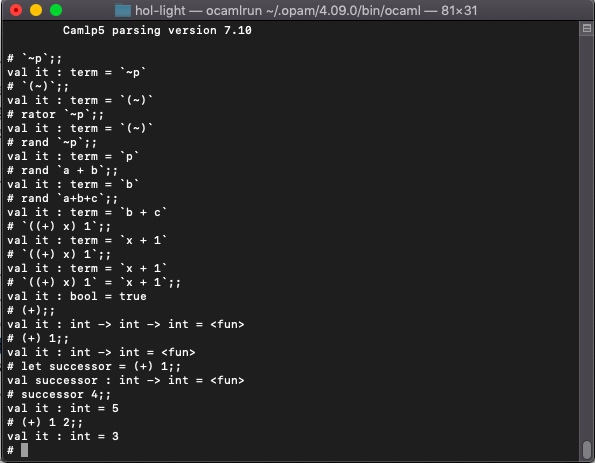
\includegraphics[width=6.2in,height=4.82in]{./media/image18.png}
	\end{FlushLeft}\end{figure}


%%%%%%%%%%%%%%%%%%%% Figure/Image No: 12 Ends here %%%%%%%%%%%%%%%%%%%%

\par


\vspace{\baselineskip}

\vspace{\baselineskip}

\vspace{\baselineskip}


%%%%%%%%%%%%%%%%%%%% Figure/Image No: 13 starts here %%%%%%%%%%%%%%%%%%%%

\begin{figure}[H]
	\begin{FlushLeft}		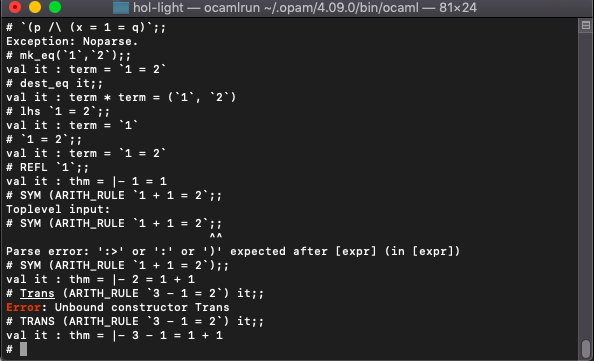
\includegraphics[width=6.19in,height=3.76in]{./media/image14.png}
	\end{FlushLeft}\end{figure}


%%%%%%%%%%%%%%%%%%%% Figure/Image No: 13 Ends here %%%%%%%%%%%%%%%%%%%%

\par


\vspace{\baselineskip}


%%%%%%%%%%%%%%%%%%%% Figure/Image No: 14 starts here %%%%%%%%%%%%%%%%%%%%

\begin{figure}[H]
	\begin{FlushLeft}		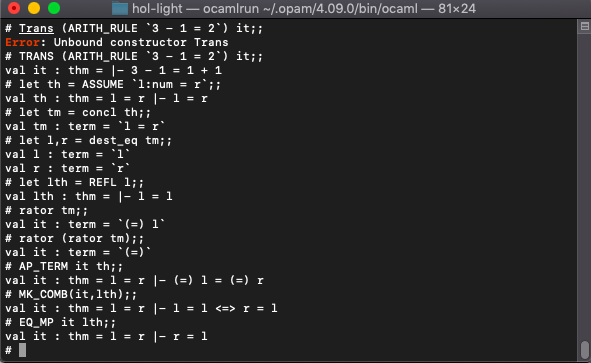
\includegraphics[width=6.16in,height=3.78in]{./media/image16.png}
	\end{FlushLeft}\end{figure}


%%%%%%%%%%%%%%%%%%%% Figure/Image No: 14 Ends here %%%%%%%%%%%%%%%%%%%%

\par


\vspace{\baselineskip}

\vspace{\baselineskip}

\vspace{\baselineskip}

\vspace{\baselineskip}

\vspace{\baselineskip}

\vspace{\baselineskip}

\vspace{\baselineskip}
\begin{FlushLeft}
{\fontsize{14pt}{16.8pt}\selectfont \textbf{08/01/2020}\par}
\end{FlushLeft}\par

{\fontsize{14pt}{16.8pt}\selectfont Studying Hol light Code:\par}\par


\vspace{\baselineskip}
{\fontsize{14pt}{16.8pt}\selectfont File name: Lib.ml\par}\par


\vspace{\baselineskip}
{\fontsize{14pt}{16.8pt}\selectfont Functions Explantion\par}\par

\href{https://www.cl.cam.ac.uk/~jrh13/hol-light/HTML/map.html}{{\fontsize{14pt}{16.8pt}\selectfont \textcolor[HTML]{1155CC}{\ul{https://www.cl.cam.ac.uk/$ \sim $ jrh13/hol-light/HTML/map.html}}}\par}\par


\vspace{\baselineskip}
{\fontsize{14pt}{16.8pt}\selectfont Starting file for hol light\par}\par

\href{https://github.com/jrh13/hol-light/blob/master/lib.ml}{{\fontsize{14pt}{16.8pt}\selectfont \textcolor[HTML]{1155CC}{\ul{https://github.com/jrh13/hol-light/blob/master/lib.ml}}}\par}\par


\vspace{\baselineskip}

\vspace{\baselineskip}
{\fontsize{14pt}{16.8pt}\selectfont Why this file Basic and advance functions mentioned this file and this is imported iin other files of hol light.\par}\par


\vspace{\baselineskip}
{\fontsize{14pt}{16.8pt}\selectfont Will start from basic to advance for better understanding of file structure in hol light.\par}\par


\vspace{\baselineskip}

\vspace{\baselineskip}
{\fontsize{14pt}{16.8pt}\selectfont \textbf{$\textbackslash$ map$\textbackslash$  -- line 48}\par}\par

{\fontsize{14pt}{16.8pt}\selectfont Takes funtion and list and appiles function to each element of list:\par}\par


\vspace{\baselineskip}


%%%%%%%%%%%%%%%%%%%% Figure/Image No: 15 starts here %%%%%%%%%%%%%%%%%%%%

\begin{figure}[H]
	\begin{Center}
		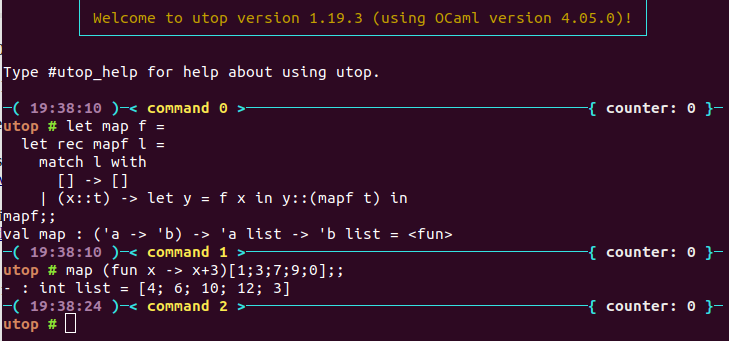
\includegraphics[width=6.27in,height=2.93in]{./media/image4.png}
	\end{Center}
\end{figure}


%%%%%%%%%%%%%%%%%%%% Figure/Image No: 15 Ends here %%%%%%%%%%%%%%%%%%%%

\par


\vspace{\baselineskip}

\vspace{\baselineskip}
{\fontsize{14pt}{16.8pt}\selectfont Showed on above example\par}\par

{\fontsize{14pt}{16.8pt}\selectfont map (fun x -> x+3)[1;3;7;9;0];;\par}\par


\vspace{\baselineskip}
{\fontsize{14pt}{16.8pt}\selectfont [4; 6; 10; 12; 3]\par}\par


\vspace{\baselineskip}
{\fontsize{14pt}{16.8pt}\selectfont \textbf{$\textbackslash$  last $\textbackslash$ --55}\par}\par



%%%%%%%%%%%%%%%%%%%% Figure/Image No: 16 starts here %%%%%%%%%%%%%%%%%%%%

\begin{figure}[H]
	\begin{Center}
		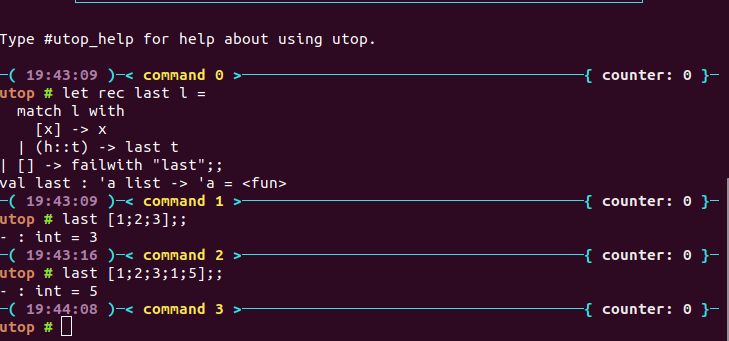
\includegraphics[width=6.27in,height=2.93in]{./media/image10.png}
	\end{Center}
\end{figure}


%%%%%%%%%%%%%%%%%%%% Figure/Image No: 16 Ends here %%%%%%%%%%%%%%%%%%%%

\par


\vspace{\baselineskip}
{\fontsize{14pt}{16.8pt}\selectfont This functions takes List and return last element of the list\par}\par

{\fontsize{14pt}{16.8pt}\selectfont and if list is empty then exception: Failure "last".\par}\par


\vspace{\baselineskip}

\vspace{\baselineskip}
{\fontsize{14pt}{16.8pt}\selectfont \textbf{$\textbackslash$  butlast $\textbackslash$  --61}\par}\par


\vspace{\baselineskip}


%%%%%%%%%%%%%%%%%%%% Figure/Image No: 17 starts here %%%%%%%%%%%%%%%%%%%%

\begin{figure}[H]
	\begin{Center}
		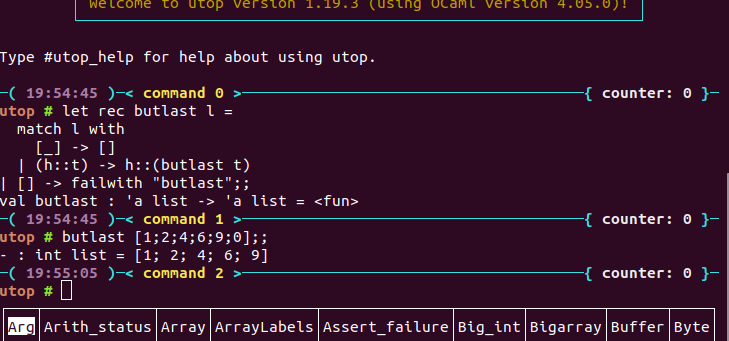
\includegraphics[width=6.27in,height=2.93in]{./media/image9.png}
	\end{Center}
\end{figure}


%%%%%%%%%%%%%%%%%%%% Figure/Image No: 17 Ends here %%%%%%%%%%%%%%%%%%%%

\par


\vspace{\baselineskip}
{\fontsize{14pt}{16.8pt}\selectfont as you can see in screenshot this function gives list except last element.\par}\par

{\fontsize{14pt}{16.8pt}\selectfont butlast [1;2;4;6;9;0];;\par}\par

{\fontsize{14pt}{16.8pt}\selectfont - : int list = [1; 2; 4; 6; 9]\par}\par


\vspace{\baselineskip}

\vspace{\baselineskip}

\vspace{\baselineskip}

\vspace{\baselineskip}

\vspace{\baselineskip}

\vspace{\baselineskip}

\vspace{\baselineskip}

\vspace{\baselineskip}

\vspace{\baselineskip}
{\fontsize{14pt}{16.8pt}\selectfont \textbf{$\textbackslash$ el $\textbackslash$  --67}\par}\par



%%%%%%%%%%%%%%%%%%%% Figure/Image No: 18 starts here %%%%%%%%%%%%%%%%%%%%

\begin{figure}[H]
	\begin{Center}
		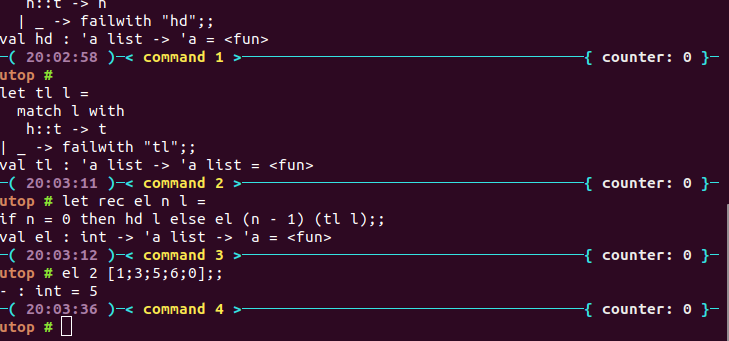
\includegraphics[width=6.27in,height=2.93in]{./media/image8.png}
	\end{Center}
\end{figure}


%%%%%%%%%%%%%%%%%%%% Figure/Image No: 18 Ends here %%%%%%%%%%%%%%%%%%%%

\par


\vspace{\baselineskip}

\vspace{\baselineskip}
{\fontsize{14pt}{16.8pt}\selectfont el function gives specfied element from list\par}\par

{\fontsize{14pt}{16.8pt}\selectfont Consist of two other function /hd/ , / tl / specifies in lib.ml\par}\par


\vspace{\baselineskip}
{\fontsize{14pt}{16.8pt}\selectfont \textbf{$\textbackslash$ rev$\textbackslash$  -- 70}\par}\par


\vspace{\baselineskip}


%%%%%%%%%%%%%%%%%%%% Figure/Image No: 19 starts here %%%%%%%%%%%%%%%%%%%%

\begin{figure}[H]
	\begin{Center}
		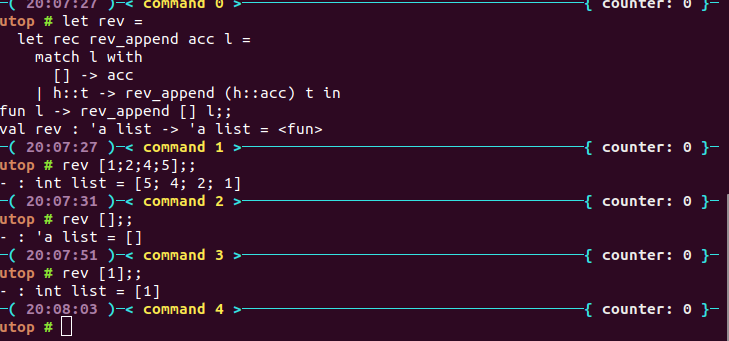
\includegraphics[width=4.34in,height=2.03in]{./media/image5.png}
	\end{Center}
\end{figure}


%%%%%%%%%%%%%%%%%%%% Figure/Image No: 19 Ends here %%%%%%%%%%%%%%%%%%%%

\par

{\fontsize{14pt}{16.8pt}\selectfont return reversed list\par}\par


\vspace{\baselineskip}
{\fontsize{14pt}{16.8pt}\selectfont \textbf{$\textbackslash$  map2 $\textbackslash$  --77 important function}\par}\par



%%%%%%%%%%%%%%%%%%%% Figure/Image No: 20 starts here %%%%%%%%%%%%%%%%%%%%

\begin{figure}[H]
	\begin{Center}
		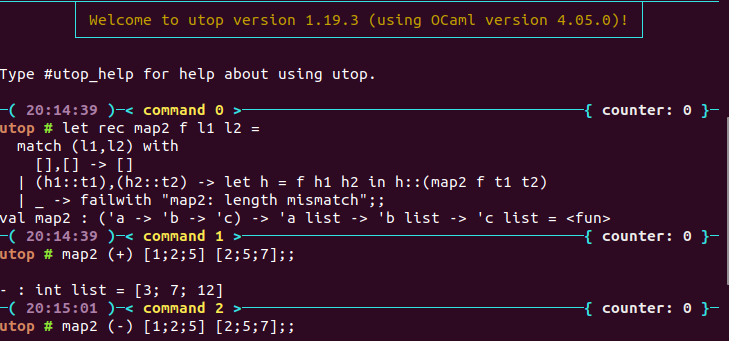
\includegraphics[width=6.27in,height=2.93in]{./media/image3.png}
	\end{Center}
\end{figure}


%%%%%%%%%%%%%%%%%%%% Figure/Image No: 20 Ends here %%%%%%%%%%%%%%%%%%%%

\par


\vspace{\baselineskip}

\vspace{\baselineskip}
{\fontsize{14pt}{16.8pt}\selectfont maps2 take two list and function and gives new list\par}\par

{\fontsize{14pt}{16.8pt}\selectfont map2 f ([x1;...;xn],[y1;...;yn]) returns [f(x1,y1);...;f(xn,yn)].\par}\par


\vspace{\baselineskip}

\vspace{\baselineskip}
{\fontsize{14pt}{16.8pt}\selectfont \textbf{$\textbackslash$ funpow $\textbackslash$  -- 95}\par}\par



%%%%%%%%%%%%%%%%%%%% Figure/Image No: 21 starts here %%%%%%%%%%%%%%%%%%%%

\begin{figure}[H]
	\begin{Center}
		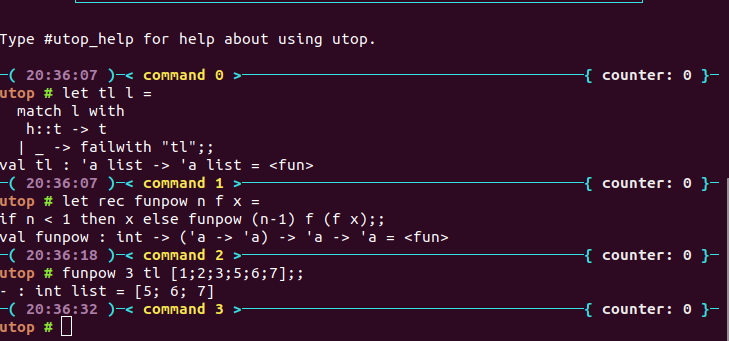
\includegraphics[width=6.27in,height=2.93in]{./media/image11.png}
	\end{Center}
\end{figure}


%%%%%%%%%%%%%%%%%%%% Figure/Image No: 21 Ends here %%%%%%%%%%%%%%%%%%%%

\par


\vspace{\baselineskip}
{\fontsize{14pt}{16.8pt}\selectfont This function takes 3 argument: int -> ('a -> 'a) -> 'a -> 'a = <fun>\par}\par

{\fontsize{14pt}{16.8pt}\selectfont how many times n a function f applies to x\par}\par


\vspace{\baselineskip}
{\fontsize{14pt}{16.8pt}\selectfont \textbf{$\textbackslash$  itlist $\textbackslash$  --112}\par}\par


\vspace{\baselineskip}

\vspace{\baselineskip}
{\fontsize{14pt}{16.8pt}\selectfont This function applies function f to adjacent element of list\par}\par



%%%%%%%%%%%%%%%%%%%% Figure/Image No: 22 starts here %%%%%%%%%%%%%%%%%%%%

\begin{figure}[H]
	\begin{Center}
		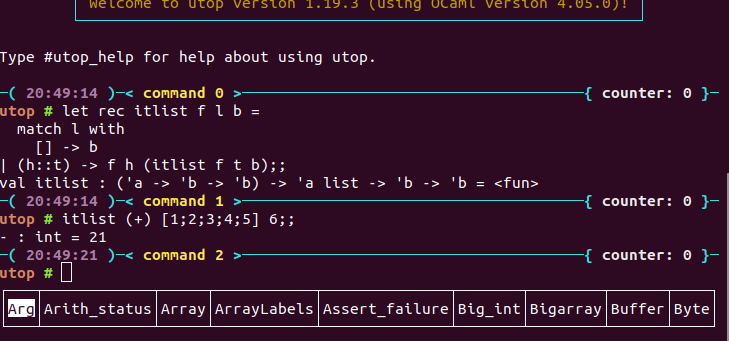
\includegraphics[width=6.27in,height=2.93in]{./media/image2.png}
	\end{Center}
\end{figure}


%%%%%%%%%%%%%%%%%%%% Figure/Image No: 22 Ends here %%%%%%%%%%%%%%%%%%%%

\par


\vspace{\baselineskip}

\vspace{\baselineskip}
{\fontsize{14pt}{16.8pt}\selectfont SET OPERATIONS ON LIST:\par}\par


\vspace{\baselineskip}
{\fontsize{14pt}{16.8pt}\selectfont \textbf{$\textbackslash$ mem$\textbackslash$  -- 263}\par}\par



%%%%%%%%%%%%%%%%%%%% Figure/Image No: 23 starts here %%%%%%%%%%%%%%%%%%%%

\begin{figure}[H]
	\begin{Center}
		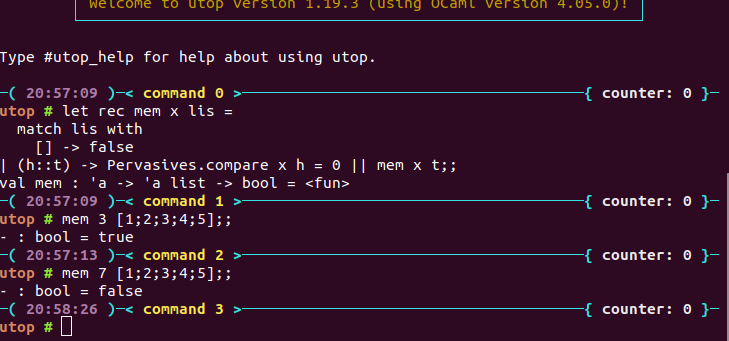
\includegraphics[width=6.27in,height=2.93in]{./media/image7.png}
	\end{Center}
\end{figure}


%%%%%%%%%%%%%%%%%%%% Figure/Image No: 23 Ends here %%%%%%%%%%%%%%%%%%%%

\par


\vspace{\baselineskip}
{\fontsize{14pt}{16.8pt}\selectfont mem is a boolen type function\par}\par

{\fontsize{14pt}{16.8pt}\selectfont returns true if given element is present in list else return false\par}\par


\vspace{\baselineskip}
{\fontsize{14pt}{16.8pt}\selectfont \textbf{$\textbackslash$  Insert$\textbackslash$ -- 268}\par}\par


\vspace{\baselineskip}
{\fontsize{14pt}{16.8pt}\selectfont insert function checks element is present in list if not the insert that element in that list\par}\par



%%%%%%%%%%%%%%%%%%%% Figure/Image No: 24 starts here %%%%%%%%%%%%%%%%%%%%

\begin{figure}[H]
	\begin{Center}
		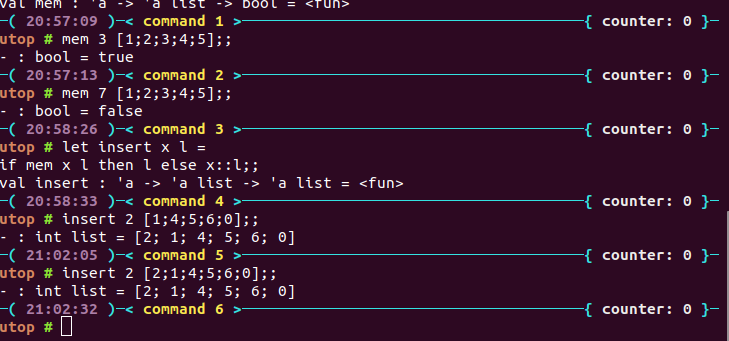
\includegraphics[width=6.27in,height=2.93in]{./media/image12.png}
	\end{Center}
\end{figure}


%%%%%%%%%%%%%%%%%%%% Figure/Image No: 24 Ends here %%%%%%%%%%%%%%%%%%%%

\par


\vspace{\baselineskip}

\vspace{\baselineskip}
{\fontsize{14pt}{16.8pt}\selectfont \textbf{$\textbackslash$ union$\textbackslash$  -- 271}\par}\par



%%%%%%%%%%%%%%%%%%%% Figure/Image No: 25 starts here %%%%%%%%%%%%%%%%%%%%

\begin{figure}[H]
	\begin{Center}
		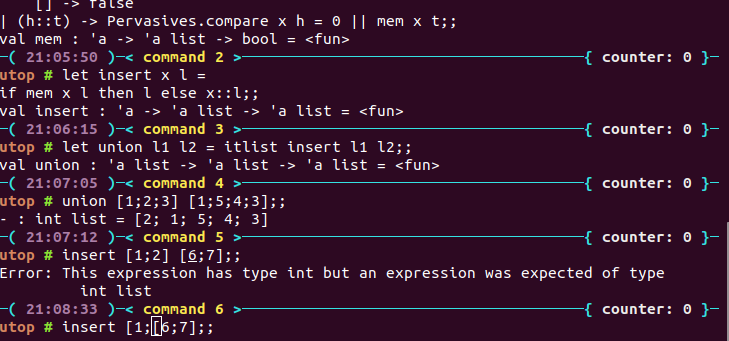
\includegraphics[width=6.27in,height=2.93in]{./media/image6.png}
	\end{Center}
\end{figure}


%%%%%%%%%%%%%%%%%%%% Figure/Image No: 25 Ends here %%%%%%%%%%%%%%%%%%%%

\par


\vspace{\baselineskip}
{\fontsize{14pt}{16.8pt}\selectfont Union returns a list consisting of the elements of l1 not already in l2 concatenated with l2\par}\par


\vspace{\baselineskip}

\vspace{\baselineskip}

\vspace{\baselineskip}

\vspace{\baselineskip}
\begin{FlushLeft}
{\fontsize{14pt}{16.8pt}\selectfont $\textbackslash$ documentclass$ \{ $ article$ \} $ \par}
\end{FlushLeft}\par


\vspace{\baselineskip}
\begin{FlushLeft}
{\fontsize{14pt}{16.8pt}\selectfont \textbf{$\textbackslash$ title$ \{ $ HOL's Notes$ \} $ }\par}
\end{FlushLeft}\par


\vspace{\baselineskip}
\begin{FlushLeft}
{\fontsize{14pt}{16.8pt}\selectfont $\textbackslash$ begin$ \{ $ document$ \} $ \par}
\end{FlushLeft}\par

\begin{FlushLeft}
{\fontsize{14pt}{16.8pt}\selectfont $\textbackslash$ maketitle\par}
\end{FlushLeft}\par


\vspace{\baselineskip}
\begin{FlushLeft}
{\fontsize{14pt}{16.8pt}\selectfont $\textbackslash$ section$ \{ $ Number System$ \} $ \par}
\end{FlushLeft}\par

\begin{FlushLeft}
{\fontsize{14pt}{16.8pt}\selectfont Hol supports several number systems\par}
\end{FlushLeft}\par


\vspace{\baselineskip}
\begin{FlushLeft}
{\fontsize{14pt}{16.8pt}\selectfont $\textbackslash$ subsection$ \{ $ Natural Numbers$ \} $ \par}
\end{FlushLeft}\par

\begin{FlushLeft}
{\fontsize{14pt}{16.8pt}\selectfont N = $\textbackslash$ big$\textbackslash$ $ \{ $ 1 , 2 , 3.....$\textbackslash$ big$\textbackslash$ $ \} $ \par}
\end{FlushLeft}\par


\vspace{\baselineskip}
\begin{FlushLeft}
{\fontsize{14pt}{16.8pt}\selectfont $\textbackslash$ subsection$ \{ $ Integers$ \} $ \par}
\end{FlushLeft}\par

\begin{FlushLeft}
{\fontsize{14pt}{16.8pt}\selectfont Z = $\textbackslash$ big$\textbackslash$ $ \{ $ ..,-2 , -1 , 0 , 1 , 2 ,..$\textbackslash$ big$\textbackslash$ $ \} $ \par}
\end{FlushLeft}\par


\vspace{\baselineskip}
\begin{FlushLeft}
{\fontsize{14pt}{16.8pt}\selectfont $\textbackslash$ subsection$ \{ $ Real Numbers$ \} $ \par}
\end{FlushLeft}\par

\begin{FlushLeft}
{\fontsize{14pt}{16.8pt}\selectfont R = $\textbackslash$ big$\textbackslash$ $ \{ $ ..,-3 , -1.2 , 0 , 1.4 , 2 , 2.4 ,..$\textbackslash$ big$\textbackslash$ $ \} $ \par}
\end{FlushLeft}\par


\vspace{\baselineskip}
\begin{FlushLeft}
{\fontsize{14pt}{16.8pt}\selectfont $\textbackslash$ paragraph$ \{ $ $ \} $  In set notation we can write it as N $\textbackslash$ subseteq Z $\textbackslash$ subseteq R .\par}
\end{FlushLeft}\par


\vspace{\baselineskip}
\begin{FlushLeft}
{\fontsize{14pt}{16.8pt}\selectfont $\textbackslash$ paragraph$ \{ $ $ \} $ \par}
\end{FlushLeft}\par

\begin{FlushLeft}
{\fontsize{14pt}{16.8pt}\selectfont However, it can sometimes be quite inconvenient that there are no negative numbers in N. In fact, HOL’s subtraction on type num is defined as ‘cutoff’ subtraction so that m - n is defined only if m $\textbackslash$ leq n.\par}
\end{FlushLeft}\par


\vspace{\baselineskip}
\begin{FlushLeft}
{\fontsize{14pt}{16.8pt}\selectfont ARITH$\textbackslash$ \_RULE $\textbackslash$ `(m - n) + n = m$\textbackslash$ `;;\par}
\end{FlushLeft}\par


\vspace{\baselineskip}
\begin{FlushLeft}
{\fontsize{14pt}{16.8pt}\selectfont Exception: Failure "linear$\textbackslash$ \_ineqs: no contradiction".\par}
\end{FlushLeft}\par


\vspace{\baselineskip}
\begin{FlushLeft}
{\fontsize{14pt}{16.8pt}\selectfont eg.ARITH$\textbackslash$ \_RULE $\textbackslash$ `(1 - 2) + 2 = 2$\textbackslash$ `;;\par}
\end{FlushLeft}\par


\vspace{\baselineskip}
\begin{FlushLeft}
{\fontsize{14pt}{16.8pt}\selectfont returns $\textbackslash$ rightarrow val $\textbackslash$ hspace$ \{ $ 0.2cm$ \} $  it : thm = $\textbackslash$ vdash 1 - 2 + 2 = 2\par}
\end{FlushLeft}\par


\vspace{\baselineskip}
\begin{FlushLeft}
{\fontsize{14pt}{16.8pt}\selectfont ARITH$\textbackslash$ \_RULE\ $\textbackslash$ `n $\textbackslash$ leq m $\textbackslash$ Rightarrow  (m - n) + n = m$\textbackslash$ `;;\par}
\end{FlushLeft}\par


\vspace{\baselineskip}
\begin{FlushLeft}
{\fontsize{14pt}{16.8pt}\selectfont returns $\textbackslash$ rightarrow val $\textbackslash$ hspace$ \{ $ 0.2cm$ \} $  it : thm = $\textbackslash$ vdash n $\textbackslash$ leq m $\textbackslash$ Rightarrow m - n + n = m\par}
\end{FlushLeft}\par


\vspace{\baselineskip}

\vspace{\baselineskip}

\vspace{\baselineskip}

\vspace{\baselineskip}

\vspace{\baselineskip}

\vspace{\baselineskip}

\vspace{\baselineskip}
\begin{FlushLeft}
{\fontsize{14pt}{16.8pt}\selectfont $\textbackslash$ end$ \{ $ document$ \} $ \par}
\end{FlushLeft}\par


\printbibliography
\end{document}